One of the most established cryptanalytic methods against block ciphers is linear cryptanalysis~\cite{Matsui1993}. These attacks are statistical in nature, in which the attacker attempts to construct probabilistic patterns through as many rounds of the cipher as possible, in order to distinguish the cipher from a random permutation, and ultimately recover the key. Due to their very nature, these attacks require a very large number of plaintext--ciphertext pairs, ensuring that (usually) they rapidly become impractical. In fact, most modern ciphers have been designed with these attacks in mind, and therefore do not generally have their security affected by them.

On the other hand, the proposal of algebraic attacks -- an explicitly non-statistical attack technique -- against block ciphers has been the source of much speculation; while a well-established technique against some stream ciphers constructions~\cite{ars-faugere:inria2005,courtois-meier:eurocrypt2003}, the viability of algebraic attacks against block ciphers remains subject to debate. On the one hand, these attack techniques promise to allow the cryptanalyst to recover secret key bits given only one or very few plaintext--ciphertext pairs. On the other hand, the runtime of algebraic attacks against block ciphers is not well understood, and it is so far not clear whether algebraic attacks can break any proposed block cipher faster than other techniques (cf. Chapter~\ref{chapter:algebraic_attacks}).

A promising approach however is to combine both statistical and algebraic techniques in block cipher cryptanalysis. In fact, many proposed algebraic approaches already involve statistical components. For instance, the equation systems usually considered for the AES~\cite{murphy-robshaw:crypto2002,alg-aes-book}, use
the \emph{inversion equation} $xy = 1$ for the S-Box. While this equation only holds with probability $p = 255/256$, it may well offer some advantages when compared with the correct equation $x^{254} = y$ representing the S-Box (which due to its very high degree, is usually considered impractical). Further recent
examples include key bit guesses \cite{alg-des}, the use of SAT-solvers \cite{bard-phd} and the Raddum-Semaev algorithm \cite{Raddum2006} for solving polynomial equations.

In this chapter we will discuss the relationship between linear cryptanalysis and algebraic attack techniques. The results in this chapter are relatively straight-forward and mainly serve as a preparation for the next chapter on algebraic techniques in differential cryptanalysis.

\section{Linear Cryptanalysis (LC)}
Linear Cryptanalysis was first introduced by Mitsuru Matsui at Eurocrypt~'93 \cite{Matsui1993} as a theoretical attack against DES. Eventually, this lead to a practical attack against DES requiring $2^{43}$ known plaintext-ciphertext pairs. Matsui introduced two algorithms in \cite{Matsui1993} numbered $1$ and $2$. Later \emph{Algorithm 2} was also referred to as 1R or 2R approach, depending on the exact setup.

\emph{Algorithm 1} works by finding linear relationships between some plaintext bits, some ciphertext
bits and some key bits.
\begin{equation}
\label{lc:algorithm1}
P_i \oplus \dots \oplus P_m \oplus C_j + \dots \oplus C_n = K_k \oplus \dots \oplus K_o
\end{equation}
If this relationship holds with a probability $p$ sufficiently bounded away from $1/2$ (i.e. it has a bias $b > 0$) this can be exploited using many plaintext-ciphertext pairs. If $T$ is the number of plaintext-ciphertext pairs such that the left hand side of equation~\ref{lc:algorithm1} is equal to zero and $N$ the number plaintext-ciphertext pairs and $T>N/2$ then guess $K_k + \dots \oplus K_o = 0$ when $p > 1/2$, or $1$ otherwise. If $T < N/2$ then guess $K_k \oplus \dots \oplus K_o = 1$ when $p > 1/2$ or $0$ otherwise. Clearly, this algorithm's complexity and success rate is determined by the number of plaintexts $N$ and the bias $b$.

\emph{Algorithm 2} works by finding linear relationships between some plaintext bits, some subkey bits and some bits from the input to the last round. If this linear relation holds with a probability sufficiently bounded away from $1/2$ (i.e. it has a bias $b > 0$) the cryptanalyst can exploit it by partial decrypting a part of the known ciphertext using a guessed partial subkey (\emph{candidate key}). We assume to get random garbage if a wrong partial subkey is chosen, i.e. some relationship which holds with probability $1/2$. The cryptanalyst will increase a counter for a candidate key if the partial decrypt matches the expectation from the linear approximation. As the linear approximation holds with a probability $p \neq 1/2$ a peak will eventually be observed for the the correct candidate key if all candidates are tested with enough plaintext-ciphertext pairs.

A gentle introduction to linear cryptanalysis is given in Howard M. Heys' tutorial \cite{Heys2002} and Mitsuru Matsui's original paper \cite{Matsui1993}. Also, many extensions of linear cryptanalysis exist such as ``Linear Cryptanalysis using Multiple Approximations'' \cite{Robshaw1994} and ``Non-Linear  Approximations in Linear Cryptanalsyis'' \cite{Knudsen1996}. However, in this chapter we only consider the most basic form of linear cryptanalysis.

\section{The Heys-Toy-Cipher (HTC)}

In order to illustrate the connection between linear and algebraic cryptanalysis, we will use  the toy cipher Heys developed for his linear and differential cryptanalysis tutorial \cite{Heys2002}. We call this cipher the Heys-Toy-Cipher (HTC). It is chosen because the reader might be familiar with it already due to the wide recognition of Heys' tutorial and because we do not have to worry about performing a linear cryptanalysis.

HTC is a basic Substitution-Permutation Network (SPN). The cipher takes a 16-bit input block and processes the block by repeating the basic operations of a round four times. Each round consists of substitution, a transposition of the bits (i.e., permutation of the bit positions), and key addition. The basic structure of the cipher is visualised in Figure~\ref{fig:htc}

\begin{figure}[ht]
 \centering
 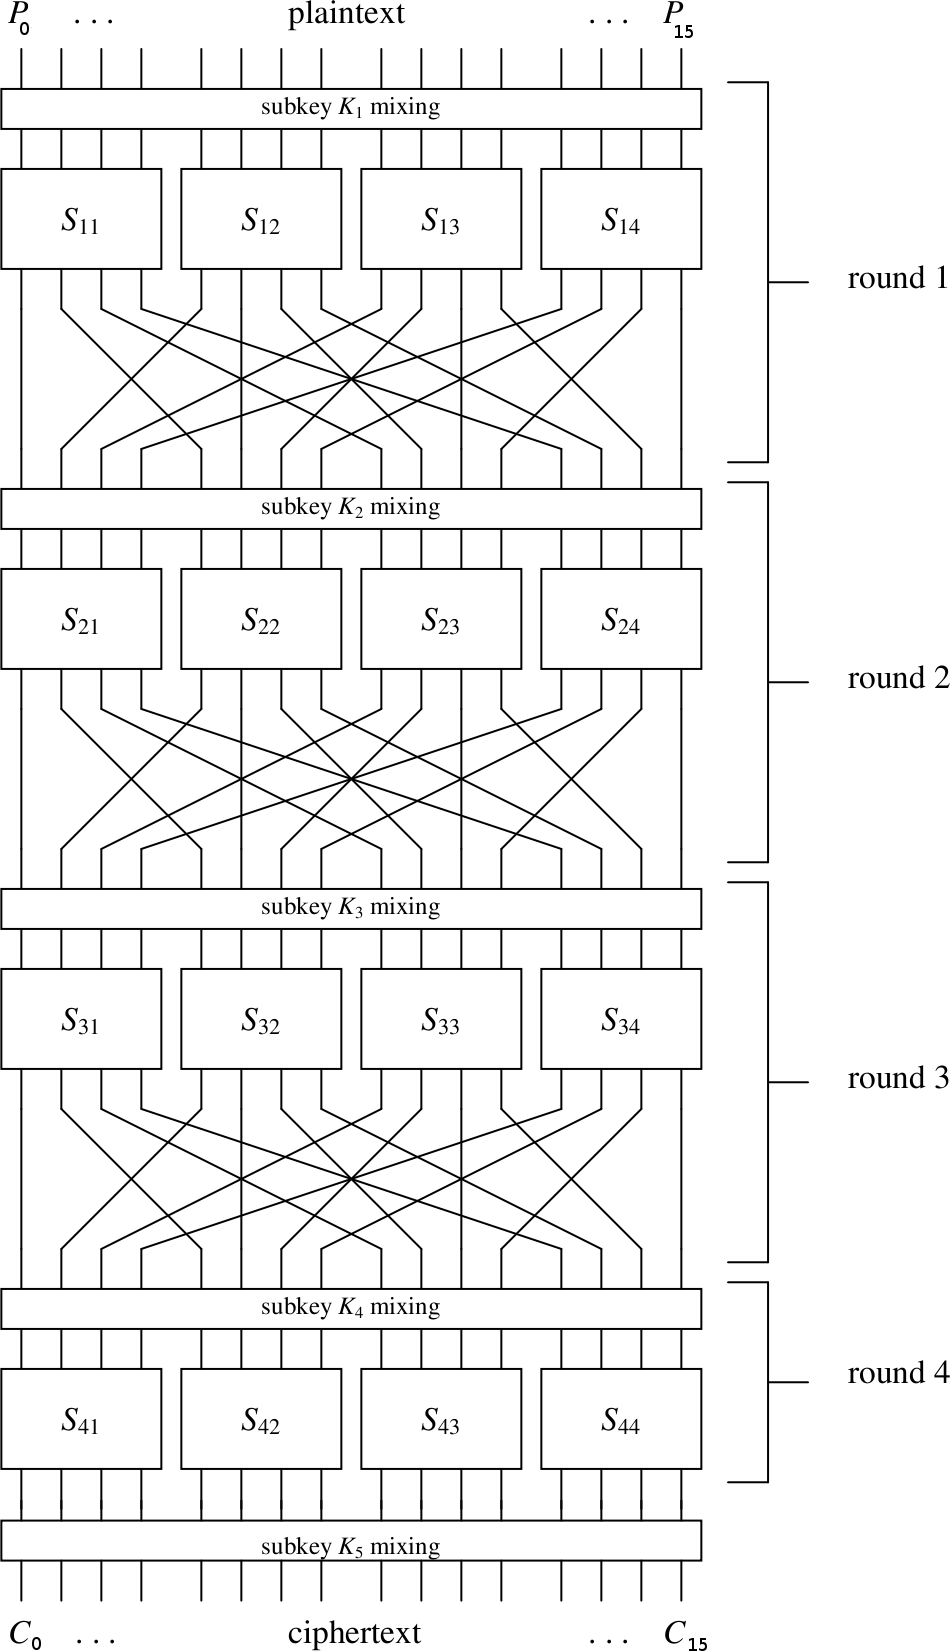
\includegraphics[height=0.6\textheight]{./heys-toy-cipher.png}
 \caption{Basic Structure of the Heys-Toy-Cipher from \cite{Heys2002}}
 \label{fig:htc}
\end{figure}


The cipher breaks the 16-bit data block into four 4-bit sub-blocks. Each sub-block forms an input to a $4\times4$ S-box (a substitution with 4 input and 4 output bits). The S-box is given by a lookup table where the most significant bit of the hexadecimal notation represents the leftmost bit of the S-box, i.e. we are using big endian notation.

\begin{center}
\begin{tabular}{|l |c|c|c|c| c|c|c|c| c|c|c|c| c|c|c|c|}
\hline
input  & 0 & 1 & 2 & 3 & 4 & 5 & 6 & 7 & 8 & 9 & A & B & C & D & E & F\\
\hline
output & E & 4 & D & 1 & 2 & F & B & 8 & 3 & A & 6 & C & 5 & 9 & 0 & 7\\
\hline
\end{tabular}
\end{center}

Alternatively, the S-box can be presented as polynomials in $\F_{2}[y_{3}, y_{2}, y_{1}, y_{0}, x_{3}, x_{2}, x_{1},
x_{0}]$ (where $x_3$ represents the least-significant input bit, $x_0$ the most-significant input bit, $y_3$ the
least-significant output bit and $y_0$ the most-significant output bit):

\begin{align*}
y_{0} =& x_{3}x_{2}x_{1} + x_{3} + x_{2} + x_{1} + x_{0} + 1,\\
y_{1} =& x_{3}x_{2}x_{0} + x_{3}x_{0} + x_{3} + x_{2}x_{1}x_{0} + x_{2}x_{0} + x_{1} + 1,\\
y_{2} =& x_{3}x_{1}x_{0} + x_{3}x_{0} + x_{2} + x_{1}x_{0} + x_{1} + 1,\\
y_{3} =& x_{3}x_{2}x_{1} + x_{3}x_{2} + x_{3}x_{1}x_{0} + x_{3}x_{0} + x_{3} + x_{2}x_{1} + x_{1}x_{0} + x_{1} + x_{0}.\\
\end{align*}

The permutation portion of a round is simply the transposition of the bits or the permutation of the bit positions. The permutation is given in the following table (where the numbers represent bit positions in the block, with 0 being the leftmost bit and 15 being the rightmost bit) and can be simply described as: the output $i$ of S-box $j$ is connected to input $j$ of S-box $i$. There would be no purpose for a permutation in the last round and, hence, the cipher does not have one. Please also note that the ordering here is little endian contrary to the big endian ordering of the S-box.

\begin{center}
\begin{tabular}{|l |c|c|c|c| c|c|c|c| c|c|c|c| c|c|c|c|}
\hline
  input  & 0 & 1 & 2 &  3 & 4 & 5 & 6 &  7 & 8 & 9 & 10 & 11 & 12 & 13 & 14 & 15 \\
\hline
output & 0 & 4 & 8 & 12 & 1 & 5 & 9 & 13 & 2 & 6 & 10 & 14 &  3 &  7 & 11 & 15 \\
\hline
\end{tabular}
\end{center}

Heys does not specify how subkeys are to be generated for the cipher so we use the identity map, i.e. each subkey is identically to the user-provided key. So the user-provided key  is added (XORed) to the output of the permutation layer and the result of this XOR is used as input for the next substitution layer.

One cipher round consists of an application of the substition layer, the permutation layer and the key addition. This is repeated four times as the cipher has four rounds. However, before the first round another key addition is performed and the fourth round does not feature a permutation.

We call $X_{i,j}$ the $j$-th bit/variable of the input of round $i$ and $Y_{i,j}$ the $j$-th output bit of the substition layer of the $i$-th round. We start counting the variables at $0$ and the rounds at $1$.


\subsection{An Equation System for the Heys-Toy-Cipher}

Constructing an equation system for the HTC is straight-forward once a polynomial representation of the S-box is found. Besides the S-box only the key addition needs to be accounted for and it is linear and thus easily represented as a set of polynomials.
                                                            
We represent the S-box by a set of 21 quadratic and 2 cubic polynomials, which form a \emph{degrevlex} Gröbner basis.

\begin{align*}
& x_{1}y_{0} + y_{3}y_{0} + y_{1}y_{0} + x_{1} + y_{3} + y_{1} + y_{0} + 1,\\
& x_{2}y_{0} + y_{2}y_{0} + y_{1}y_{0} + x_{2} + y_{2} + y_{1} + y_{0} + 1,\\
& x_{3}y_{0} + x_{0}y_{0} + y_{3}y_{0} + x_{2} + x_{1} + y_{3} + y_{2} + y_{0},\\
& x_{0}y_{1} + y_{3}y_{1} + y_{2}y_{1} + y_{1}y_{0} + x_{0} + y_{3} + y_{2} + y_{1} + y_{0} + 1,\\
& x_{1}y_{1} + y_{3}y_{1} + x_{0}y_{0} + y_{2}y_{0} + x_{2} + y_{2} + y_{1} + 1,\\
& x_{2}y_{1} + y_{2}y_{1} + y_{1}y_{0},\\
& x_{3}y_{1} + y_{3}y_{1} + y_{2}y_{1} + y_{1},\\
& y_{3}y_{2} + y_{2}y_{1} + x_{3} + x_{2} + x_{0} + y_{1},\\
& x_{0}y_{2} + y_{2}y_{0} + x_{3} + x_{2} + y_{3} + y_{2} + y_{0} + 1,\\
& x_{2}y_{2} + y_{2}y_{1} + x_{0}y_{0} + y_{1}y_{0} + x_{1} + y_{3} + y_{1} + 1,\\
& x_{3}y_{2} + x_{0}y_{0} + y_{2}y_{0} + y_{1}y_{0} + x_{1} + x_{0} + y_{2} + y_{0},\\
& x_{0}y_{3} + y_{3}y_{1} + y_{2}y_{1} + y_{3}y_{0} + x_{3} + x_{2} + y_{3} + y_{2} + y_{0} + 1,\\
& x_{1}y_{3} + y_{3}y_{1} + x_{0}y_{0} + y_{2}y_{0} + y_{1}y_{0},\\
& x_{2}y_{3} + y_{3}y_{1} + y_{2}y_{1} + y_{3}y_{0} + x_{3} + x_{2} + x_{0} + y_{3} + y_{1},\\
& x_{3}y_{3} + y_{3}y_{1} + y_{2}y_{1} + x_{3} + x_{2} + x_{0} + y_{3} + y_{1},\\
& x_{1}x_{0} + x_{1}y_{2} + y_{3}y_{0} + x_{2} + x_{0} + y_{1} + 1,\\
& x_{2}x_{0} + y_{3}y_{1} + y_{2}y_{1} + x_{3} + x_{2} + x_{1} + y_{3} + 1,\\
& x_{3}x_{0} + y_{3}y_{0} + y_{2}y_{0} + y_{1}y_{0} + x_{0} + y_{3} + y_{2} + y_{1} + y_{0} + 1,\\
& x_{2}x_{1} + x_{1}y_{2} + y_{3}y_{1} + y_{3}y_{0} + x_{1},\\
& x_{3}x_{1} + x_{1}y_{2} + y_{1}y_{0} + x_{3} + x_{2} + y_{3} + 1,\\
& x_{3}x_{2} + y_{3}y_{1} + y_{2}y_{1} + y_{3}y_{0} + y_{2}y_{0} + y_{1}y_{0} + x_{3} + x_{0} + y_{3} + y_{2} + y_{0} + 1,\\
& y_{2}y_{1}y_{0} + x_{1}y_{2} + y_{2}y_{0} + x_{3} + x_{2} + x_{0} + y_{2} + y_{1},\\
& y_{3}y_{1}y_{0} + y_{3}y_{0} + y_{1}y_{0} + x_{2} + y_{2} + y_{1} + 1.\\
\end{align*}

A HTC instance with $N_r$ rounds thus has $(N_r + 1) \cdot 16$ linear equations for the key additions, $N_r \cdot 4
\cdot 21$ quadratic equations and $N_r \cdot 4 \cdot 2$ cubic equations. These equations are in $16 + 2 \cdot N_r \cdot
16$ variables. Thus a four-round standard instance gives rise to $448$ equations in $144$ variables. We also add the
field equations to the set of equation and thus end up with a system of $592$ equations in $144$ variables. A three
round variant gives rise to a system with $452$ equations in $112$ variables.

\subsection{Linear Approximations}
Using a linear approximation matrix (cf.~\cite{Heys2002}) the following probabilistic linear equations can be found for the S-box:

Four linear equations are true with probability $0.875$:
\begin{align*}
0 &= x_{3} + y_{3} + y_{2} + y_{1} & 0 &= x_{2} + y_{2} + y_{1} + y_{0} + 1,\\
0 &= x_{3} + x_{2} + y_{3} + y_{0} + 1 & 0 &= x_{0} + y_{3} + y_{2} + y_{1} + y_{0} + 1.\\
\end{align*}

24 linear equations are true with probability $0.75$:
\begin{align*}
0 &= x_{1} + y_{3} + y_{1} + 1, & 0 &= x_{1} + y_{3} + y_{1} + y_{0} + 1,\\
0 &= x_{3} + x_{1} + y_{2} + y_{1}, & 0 &= x_{3} + x_{1} + y_{2} + y_{0} + 1,\\
0 &= x_{2} + x_{1} + y_{3} + y_{2}, & 0 &= x_{2} + x_{1} + y_{3} + y_{2} + y_{0},\\
0 &= x_{3} + x_{2} + x_{1} + y_{3} + y_{1} + 1, & 0 &= x_{3} + x_{2} + x_{1} + y_{1} + y_{0},\\
0 &= x_{3} + x_{0} + y_{0} + 1, & 0 &= x_{3} + x_{0} + y_{3} + y_{1} + y_{0},\\
0 &= x_{2} + x_{0} + y_{3}, & 0 &= x_{2} + x_{0} + y_{1} + 1,\\
0 &= x_{3} + x_{2} + x_{0} + y_{3}, & 0 &= x_{3} + x_{2} + x_{0} + y_{3} + y_{2} + 1,\\
0 &= x_{3} + x_{2} + x_{0} + y_{1}, & 0 &= x_{3} + x_{2} + x_{0} + y_{2} + y_{1},\\
0 &= x_{1} + x_{0} + y_{2}, & 0 &= x_{1} + x_{0} + y_{3} + y_{2} + y_{0},\\
0 &= x_{3} + x_{1} + x_{0} + y_{3} + y_{1}, & 0 &= x_{3} + x_{1} + x_{0} + y_{0} + 1,\\
0 &= x_{2} + x_{1} + x_{0} + y_{3} + y_{1} + 1, & 0 &= x_{2} + x_{1} + x_{0} + y_{1} + y_{0} + 1,\\
0 &= x_{3} + x_{2} + x_{1} + x_{0} + y_{2} + 1, & 0 &= x_{3} + x_{2} + x_{1} + x_{0} + y_{2} + y_{0}.
\end{align*}


\section{Linear Cryptanalysis in Algebraic Terms}
First, consider Matsui's \emph{Algorithm 1}. Essentially, a very simple probabilistic linear equation system is solved by evaluating it at enough data points. That is we compute $N$ varieties and check where they intersect most\footnote{Without lost of generality we may assume that we are looking for the point where they intersect most as we can simply add $1$ to one side of an equations.}. This intersection check is performed by incrementing counters for the respective varieties. 

Now, consider \emph{Algorithm 2}. In this variant a probabilistic linear relationship of the last round is replaced by a higher-order relationship true with probability $1$, while the probabilistic relations from the previous rounds remain. As a result more key bit information is available and only $R-1$ approximations are necessary. The 2R variant does the same for the first and the last round of the cipher. The cost of this transition however is that a more difficult systems have to be solved. In Matsui's paper and in linear cryptanalysis in general these systems are solved using brute force by trying all possible candidate keys. This is a reasonable approach because the search space is small.

Later, Knudsen and Robshaw \cite{Knudsen1996} pushed this idea further by explicitly adding probabilistic non-linear equations to the system. The advantage of this idea is that these might have higher probability than linear approximations but lower degree and fewer variables than the correct relationships. However, this approach poses a problem. Non-linear equations are not as easily XORed as linear equations in the sense that intermediate variables cancel out. Thus, it is more difficult to apply the \emph{Piling-Up} lemma (cf.~\cite{Heys2002}). Therefore \cite{Knudsen1996} restricts non-linear approximations to the outer rounds.

In algebraic cryptanalysis on the other hand the attacker considers polynomial systems which are always correct and tries to solve them using sophisticated means. However, as systems in linear cryptanalysis became more sophisticated researchers in algebraic cryptanalysis simplified their systems in order to gain better attacks. Examples of this trend are guessed key bits and BES-style equation systems for the AES \cite{murphy-robshaw:crypto2002} where the relationship $y = x^{254}$ is represented as $1 = xy$ which holds with probability $\frac{255}{256}$.

We can parameterise both attacks as follows: Let $F$ be a (potentially linear) polynomial system of equations, let $e$ be an estimation of the complexity of solving $F$, let $p$ be the probability an instance of $F$ is correct and $N$ the number of required (chosen or known) plaintext-ciphertext pairs. 

\begin{table}[htbp]
\begin{center}
\begin{tabular}{|l|c|c|c|}
\hline
Attack & $e$ & $p$ & $N$\\
\hline
Algebraic & $\ord{2^n}$ & $\approx 1$ & $\ord{1}$\\
Linear & $\ord{1}$ & $0 < p\neq 1/2 < 1$ & $\ord{1/|p -1/2|^2}$\\
\hline
\end{tabular}
\end{center}
\caption{Algebraic and linear attacks in comparison for an $n$-bit key.}
\label{tab:linalg-comp}
\end{table}

Thus, by increasing $N$ we can decrease $e$ (and vice versa) and we are faced with the optimisation problem where we modify different parameters in order to get an efficient attack. However, we need to translate linear cryptanalysis to algebraic terms first to show that such a balanced algorithm exists.

\subsection{Linear Cryptanalysis as an Algebraic Attack}
Consider Heys' Toy Cipher and a 1R linear cryptanalysis. First, a linear approximation of the first three rounds needs to
be found. \cite{Heys2002} uses four linear equations which are true with probability $<1$ to mount a linear cryptanalysis. These are:
\begin{align*}
0 &= Y_{1, 5} + X_{1, 4} + X_{1, 6} + X_{1,7}\\
0 &= Y_{2, 5} + Y_{2, 7} + X_{2, 5} + 1 \\
0 &= Y_{3, 5} + Y_{3, 7} + X_{3, 5} + 1 \\
0 &= Y_{3,13} + Y_{3,15} + X_{3,13} + 1 \\ 
\end{align*}

We added $1$ to those equations which are true with a negative bias to make sure they have a positive bias.
Each of those is true with $p=0.75$ and consequently they are all true with probability $0.75^{4} \simeq  0.32$ under the assumption they are independent. By using the Piling-Up Lemma (cf.~\cite{Matsui1993}, \cite{Heys2002}) the
sum 
\[
X_{4,5} + X_{4,7} + X_{4,13} + X_{4,15} +  P_{4} + P_{6} + P_{7} + K_{4} + K_{15} + 1
\]
of the right hand sides of these equations and the intermediate linear polynomials is equal to zero with probability
$0.53125$.

As this is a relationship between some plaintext bits and some bits from the input of the fourth round ($X_{4,j}$) which holds with a certain bias -- subject to the sum of $K_{4}$ and $K_{15}$ -- \emph{Algorithm 2} proceeds by trying all candidate keys ($K_{4}$, $K_{5}$, $K_{6}$, $K_{7}$, $K_{12}$, $K_{13}$, $K_{14}$, $K_{15}$) to decrypt the known ciphertext. If $X_{4,5} + X_{4,7} + X_{4,13} + X_{4,15}$ matches $P_{4} + P_{6} + P_{7}  + K_{4} + K_{15} + 1$ a counter for the used candidate key is incremented. If this is done often enough, we expect to see a peak for the correct candidate key.                                                                                                                                                                                                                                                                                                                                                                    

To replicate the same using Gröbner basis algorithms we simply add our equations for the two missing S-boxes and the final key addition. We call the resulting system $F$. If we subsitute the candidate keys in $F$ and compute a Gröbner basis we can check if the equation system is satisfiable, i.e. the Gröbner basis $\neq \{1\}$. If the Gröbner basis is $\neq \{1\}$ we increment a count for the considered candidate key and proceed. Otherwise, we do not increment the counter. We can avoid the candidate key substitution step by studying the symbolic Gröbner basis and incrementing a counter for each solution restricted to $K_{4}$, $K_{5}$, $K_{6}$, $K_{7}$, $K_{12}$, $K_{13}$, $K_{14}$, $K_{15}$.

The equation system we attempt to solve in this case is given 
\begin{enumerate} 
 \item by the linear approximation
\begin{align*}
0 =& X_{4,5} + X_{4,7} + X_{4,13} + X_{4,15} + K_{4} + K_{15} + P_5 + P_7 + P_8,\\
\end{align*}
\item the S-Box equations for the last round and
\begin{align*}
0 =& X_{4,4}X_{4,5}X_{4,6} + X_{4,4} + X_{4,5} + X_{4,6} + X_{4,7} + Y_{4,7} + 1, \\
0 =& X_{4,4}X_{4,5}X_{4,7} + X_{4,4}X_{4,7} + X_{4,4} + X_{4,5}X_{4,6}X_{4,7} + X_{4,5}X_{4,7} + X_{4,6} + Y_{4,6} + 1, \\
0 =& X_{4,4}X_{4,6}X_{4,7} + X_{4,4}X_{4,7} + X_{4,5} + X_{4,6}X_{4,7} + X_{4,6} + Y_{4,5} + 1, \\
0 =& X_{4,4}X_{4,5}X_{4,6} + X_{4,4}X_{4,5} + X_{4,4}X_{4,6}X_{4,7} + X_{4,4}X_{4,7} + X_{4,4}  \\
&  + X_{4,5}X_{4,6} + X_{4,6}X_{4,7} + X_{4,6} + X_{4,7} + Y_{4,4}, \\
\\
0 =& X_{4,12}X_{4,13}X_{4,14} + X_{4,12} + X_{4,13} + X_{4,14} + X_{4,15} + Y_{4,15} + 1, \\
0 =& X_{4,12}X_{4,13}X_{4,15} + X_{4,12}X_{4,15} + X_{4,12} + X_{4,13}X_{4,14}X_{4,15} + X_{4,13}X_{4,15} + X_{4,14} + Y_{0414} + 1, \\
0 =& X_{4,12}X_{4,14}X_{4,15} + X_{4,12}X_{4,15} + X_{4,13} + X_{0414}X_{0415} + X_{4,14} + Y_{4,13} + 1, \\
0 =& X_{4,12}X_{4,13}X_{4,14} + X_{4,12}X_{4,13} + X_{4,12}X_{4,14}X_{4,15} + X_{4,12}X_{4,15} \\
& + X_{4,12}  + X_{4,13}X_{4,14} + X_{4,14}X_{4,15} + X_{4,14} + X_{4,15} + Y_{4,12}, \\
\end{align*}
\item the final key addition
\begin{align*}
0 =& Y_{4,4} + K_{4} + C_4, & 0 =& Y_{4,5} + K_{5} + C_5, & 0 =& Y_{4,6} + K_{6} + C_6, & 0 =& Y_{4,7} + K_{7} + C_7,\\
0 =& Y_{4,12} + K_{12} + C_{12}, & 0 =& Y_{4,13} + K_{13} + C_{13}, & 0 =& Y_{4,14} + K_{14} + C_{14}, & 0 =& Y_{4,15} +
K_{15} + C_{15}.\\
\end{align*}
\end{enumerate}
We also add some field equations to restrict the variety to the base field.

The attacker now can increase $e$ as introduced before by setting up a more complicated equation system. For example
this 1R attack can be extended to a 2R attack by replacing the linear approximation of
first round S-Box with the correct cubic equation. Furthermore, we may want to insert the correct equations
for the S-Box in the second round. As $Y_{2,5}$ depends on all of $X_{2,4} \dots X_{2,7}$ this implies inserting
the correct cubic equations for $Y_{1,1}$,$Y_{1,5}$,$Y_{1,9}$,$Y_{1,13}$ as well. If we continue this
approach up to the penultimate round we end up with the full correct equation system.

Thus by adding more correct equations we increase $e$ but decrease $N$ and increase $p$. An alternative approach is not
to \emph{replace} linear approximations but still to \emph{add} correct equations.

\subsection{Enhancing Algebraic Attacks with Linear Cryptanalysis}

The standard strategy for simplifying an equation system in algebraic cryptanalysis is to guess key bits. The time saved during a single Gröbner basis or similar 
calculation is -- up to some number of guesses $g$ -- much greater than the addition time that is required -- by guessing $2^{g}$ times.

However, using the linear approximations arising from linear cryptanalysis we might able to do better: Guessing a linear eqution that holds with probability $p > 0.5$ is better than guessing a relationship between key variables and values which holds with probability $p = 0.5$.

\subsubsection{Experiments with Toy Instances}
\label{sec:experiments}
All experiments were carried out using the computer algebra system \Sage 2.7 \cite{sage} and the $F_4$ algorithm (cf.~Chapter~\ref{chapter:f4}) implemented in \Magma 2.13-5 \cite{magma}.

In the Tables~\ref{tab:exp-3-rounds} and \ref{tab:exp-4-rounds}, the symbol $\#$ represents the number of trials, $N_r$ represents the number of rounds, $b$ the bias of the approximations, $r$ the experimental success rate and $t$ the average time it took to compute a Gröbner basis. The estimated success rate (``est. $r$'') is computed by taking the probability of the approximates to the power of the number of the approximation, i.e. it estimates the success rate if those approximations are independent and if exactly one solution exists for the system. The quotient $t/r$ indicates the time it would take to attack the system using the given approximation.

All experiments were carried out on a 2.33~GHz Intel \CTD notebook with 2GB RAM unless stated otherwise. To carry out these experiments the number of rounds had to be reduced to $3$ in many cases because we ran out of RAM if 4 rounds were to be used without any approximations.

The polynomial ring used during all three-round experiments is

\begin{align*}
P = \F_{2}[&X_{1,0}, \dots, X_{1,15}, Y_{1,0}, \dots, Y_{1,15}, X_{2,0}, \dots, X_{2,15}, Y_{2,0}, \dots, Y_{2,15}, \\
&X_{3,0}, \dots, X_{3,15}, Y_{3,0}, \dots, Y_{3,15}, K_{0}, \dots, K_{15}].\\
\end{align*}

First, the time to compute a \emph{degrevlex} Gröbner basis without any approximations was recorded. It takes approximately 40 seconds on our system. Next, up to 5 key variables were guessed. We note that the actual success rate is always greater than the estimated success rates which can be accounted for by the fact that the system does not necessarily have only one solution.

Next, an approximation with a very high probability is chosen: $x_2 + x_3 + y_0 + y_3 + 1$ is true with probability $0.875$. Two S-Boxes per round were approximated using this linear polynomial and we see a successrate of over 50\%.

However, this approximation does not necessarily give better results than simply guessing key-bits. The next approach is to use the same linear approximation polynomials used in Heys'  linear cryptanalysis \cite{Heys2002}. Afterwards the sum -- i.e. a relationship between plaintext, ciphertext and some key bits -- as presented for linear cryptanalysis is used.

Finally, an approximation which we believed to be a ``good'' approximation is used. It is deemed ``good'' because it has high probability and is spread throughout the cipher. Indeed, it seems to provide the best results at 8.68 seconds of estimated attack time.

\begin{table}[ht]
\begin{small}
\begin{center}
\begin{tabular}{|c|r|l|c|c|c|r|r|}
\hline
\#	& $N_r$ & Approximations & $b$ & $r$ & est. $r$ & $t$ & $t$ / $r$\\
\hline

25 & 3 & -- & 0 & 1 & 1 & 40.64 & 40.64\\

\hline % guessed key bits

25 & 3 & $K_{0}$				& 0 & 0.64 & 0.5 & 30.40	 & 47.50\\
\hline
25 & 3 & $K_{0},K_{1}$			& 0 & 0.44 & 0.25 & 12.57 & 28.57\\
\hline
50 & 3 & $K_{0},K_{1},K_{2}$		& 0 & 0.28 & 0.13 & 4.74 & 16.93\\
\hline
50 & 3 & $K_{0},K_{1},K_{2},K_{3}$	& 0 & 0.16 & 0.06 & 2.46 & 15.38\\
\hline
50 & 3 & $K_{0},K_{1},K_{2},K_{3},K_{4}$	& 0 & 0.04 & 0.03 & 1.25 & 31.25\\

\hline % high probability approximation

50 & 3 &  $X_{1, 2} + X_{1, 3} + Y_{1, 0} + Y_{1, 3}$ + 1 & 0.38 & 0.58 & 0.45 & 12.77 & 22.02\\
   &   &  $X_{1,14} + X_{1,15} + Y_{1,12} + Y_{1,15}$ + 1 & & & & & \\
   &   &  $X_{2, 2} + X_{2, 3} + Y_{2, 0} + Y_{2, 3}$ + 1 & & & & & \\
   &   &  $X_{2,14} + X_{2,15} + Y_{2,12} + Y_{2,15}$ + 1 & & & & & \\
   &   &  $X_{3, 2} + X_{3, 3} + Y_{3, 0} + Y_{3, 3}$ + 1 & & & & & \\
   &   &  $X_{3,14} + X_{3,15} + Y_{3,12} + Y_{3,15}$ + 1 & & & & & \\

\hline   % linear cryptanalysis single

50 & 3 & $Y_{1, 5} + X_{1, 4} + X_{1, 6} + X_{1, 7}$ & 0.25 & 0.5 & 0.31 & 7.89 & 15.78\\
   &   & $Y_{2, 5} + Y_{2, 7} + X_{2, 5} + 1$ & & & & & \\
   &   & $Y_{3, 5} + Y_{3, 7} + X_{3, 5} + 1$ & & & & & \\
   &   & $Y_{3,13} + Y_{3,15} + X_{3,13} + 1$ & & & & & \\

\hline % linear cryptanalysis piling-up
25 & 3 & $K_{4} + K_{15} + P_{4} + P_{6} + P_{7} +$ & 0.53 & 0.64 & 0.53 & 28.58 & 44.65\\
   &   & $C_{5} + C_{7} + C_{13} + C_{15} + 1$ & & & & & \\

\hline % good approximation

50 & 3 & $X_{1, 0} + X_{1, 3} + Y_{1, 0} + 1$ & 0.25 & 0.16	& 0.08 & 1.64 &10.25\\
   &   & $X_{1, 4} + X_{1, 7} + Y_{1, 4} + 1$ & & & & & \\
   &   & $X_{1,12} + X_{1,15} + Y_{1,12} + 1$ & & & & & \\
   &   & $X_{2, 0} + X_{2, 3} + Y_{2, 0} + 1$ & & & & & \\
   &   & $X_{2, 4} + X_{2, 7} + Y_{2, 4} + 1$ & & & & & \\
   &   & $X_{2,12} + X_{2,15} + Y_{2,12} + 1$ & & & & & \\
   &   & $X_{3, 0} + X_{3, 3} + Y_{3, 0} + 1$ & & & & & \\
   &   & $X_{3, 4} + X_{3, 7} + Y_{3, 4} + 1$ & & & & & \\
   &   & $X_{3,12} + X_{3,15} + Y_{3,12} + 1$ & & & & & \\

\hline

50 & 3 & $X_{1, 0} + X_{1, 3} + Y_{1, 0} + 1$ & 0.25 & 0.4 & 0.18 & 3.47 &8.68\\
   &   & $X_{1,12} + X_{1,15} + Y_{1,12} + 1$ & & & & & \\
   &   & $X_{2, 0} + X_{2, 3} + Y_{2, 0} + 1$ & & & & & \\
   &   & $X_{2,12} + X_{2,15} + Y_{2,12} + 1$ & & & & & \\
   &   & $X_{3, 0} + X_{3, 3} + Y_{3, 0} + 1$ & & & & & \\
   &   & $X_{3,12} + X_{3,15} + Y_{3,12} + 1$ & & & & & \\

\hline

50 & 3 & $X_{1, 0} + X_{1, 3} + Y_{1, 0} + 1$ & 0.25 & 0.56 & 0.31 & 6.42 & 11.46\\
   &   & $X_{1,12} + X_{1,15} + Y_{1,12} + 1$ & & & & & \\
   &   & $X_{2, 0} + X_{2, 3} + Y_{2, 0} + 1$ & & & & & \\
   &   & $X_{2,12} + X_{2,15} + Y_{2,12} + 1$ & & & & & \\

\hline

25 & 3 & $X_{1, 0} + X_{1, 3} + Y_{1, 0} + 1$ & 0.25 & 0.84 & 0.56 & 17.28 & 20.57\\
   &   & $X_{1,12} + X_{1,15} + Y_{1,12} + 1$ & & & & & \\

\hline
\end{tabular}
\end{center}
\end{small}
\caption{Experimental results for three rounds of HTC.}
\label{tab:exp-3-rounds}
\end{table}

Table~\ref{tab:exp-4-rounds} mounts the best attack from the 3-round cipher against a 4-round cipher. We end up with
an estimated attack time of roughly 200 seconds.

\begin{table}[ht]
\begin{small}
\begin{center}
\begin{tabular}{|c|r|c|c|c|c|r|r|}
\hline
\#	& $N_r$ & Approximations & $b$ & $r$ & est. $r$ & $t$ & $t$ / $r$\\
\hline
50 & 4 & $X_{1, 0} + X_{1, 3} + Y_{1, 0} + 1$ & 0.25 & 0.26 & 0.1 & 50.9 & 195.77\\
   &   & $X_{1,12} + X_{1,15} + Y_{1,12} + 1$ & & & & & \\
   &   & $X_{2, 0} + X_{2, 3} + Y_{2, 0} + 1$ & & & & & \\
   &   & $X_{2,12} + X_{2,15} + Y_{2,12} + 1$ & & & & & \\
   &   & $X_{3, 0} + X_{3, 3} + Y_{3, 0} + 1$ & & & & & \\
   &   & $X_{3,12} + X_{3,15} + Y_{3,12} + 1$ & & & & & \\
   &   & $X_{4, 0} + X_{4, 3} + Y_{4, 0} + 1$ & & & & & \\
   &   & $X_{4,12} + X_{4,15} + Y_{4,12} + 1$ & & & & & \\
\hline
50 & 4 & $X_{1, 0} + X_{1, 3} + Y_{1, 0} + 1$ & 0.25 & 0.22 & 0.18 &118.0	& 536.36\\
   &   & $X_{1,12} + X_{1,15} + Y_{1,12} + 1$ & & & & & \\
   &   & $X_{2, 0} + X_{2, 3} + Y_{2, 0} + 1$ & & & & & \\
   &   & $X_{2,12} + X_{2,15} + Y_{2,12} + 1$ & & & & & \\
   &   & $X_{3, 0} + X_{3, 3} + Y_{3, 0} + 1$ & & & & & \\
   &   & $X_{3,12} + X_{3,15} + Y_{3,12} + 1$ & & & & & \\
\hline
\end{tabular}
\end{center}
\end{small}
\caption{Experimental results for four rounds of HTC.}
\label{tab:exp-4-rounds}
\end{table}

We also computed a \emph{degrevlex} Gröbner basis for a full four-round HTC instance on William Stein's old \url{sage.math.washington.edu} machine\footnote{purchased National Science Foundation under Grant No. 0555776} which has 64GB RAM and 16 1.8~Ghz \Opteron processors. It took 55049s (= 15.3h) cputime to compute this Gröbner basis while -- for comparison -- it took 60s cputime to compute a Gröbner basis for a three round cipher. The three round computation takes approximately 40s on the 2.33~Ghz \CTD machine.

\section{Final Remarks}
Of course, all these ``attacks'' are ridiculously inefficient when compared to a simple linear cryptanalysis or even a brute force attack. However, they do demonstrate the point that considering linear approximations may be beneficial when compared to simply guessing key bits in algebraic cryptanalysis.